\PassOptionsToPackage{dvipsnames,svgnames,x11names}{xcolor}
\documentclass[tikz,border=8pt]{standalone}
\usetikzlibrary{arrows.meta,positioning,calc,shapes,shadows,decorations.pathmorphing,shapes.geometric,backgrounds,decorations.markings,decorations.pathreplacing,decorations.text,fit,shapes.misc,shapes.arrows,matrix,bending,3d,chains,intersections,shapes.symbols,svg.path,shapes.multipart,snakes,shapes.callouts,angles,quotes}
\providecolor{gold}{RGB}{212,175,55}
\providecolor{silver}{RGB}{192,192,192}
\providecolor{bronze}{RGB}{205,127,50}
\providecolor{darkblue}{RGB}{0,0,139}
\providecolor{lightblue}{RGB}{173,216,230}
\providecolor{darkgreen}{RGB}{0,100,0}
\providecolor{lightgreen}{RGB}{144,238,144}
\providecolor{darkred}{RGB}{139,0,0}
\providecolor{navy}{RGB}{0,0,128}
\providecolor{skyblue}{RGB}{135,206,235}
\providecolor{beige}{RGB}{245,245,220}
\providecolor{cream}{RGB}{255,253,208}
\usepackage{amsmath}
\usepackage{amssymb}
\usepackage{fontawesome5}
\usetikzlibrary{fadings,shadows.blur,patterns,patterns.meta}

\providecolor{gold}{RGB}{212,175,55}
\providecolor{silver}{RGB}{192,192,192}
\providecolor{bronze}{RGB}{205,127,50}
\providecolor{darkblue}{RGB}{0,0,139}
\providecolor{lightblue}{RGB}{173,216,230}
\providecolor{darkgreen}{RGB}{0,100,0}
\providecolor{lightgreen}{RGB}{144,238,144}
\providecolor{darkred}{RGB}{139,0,0}
\providecolor{navy}{RGB}{0,0,128}
\providecolor{skyblue}{RGB}{135,206,235}
\providecolor{beige}{RGB}{245,245,220}
\providecolor{cream}{RGB}{255,253,208}

\usepackage{amsmath}
\usepackage{amssymb}
\usepackage{fontawesome5}
\usepackage{xcolor}

% --- Brand & Semantic Color Palette ---
\definecolor{domColor}{RGB}{31, 110, 165}
\definecolor{payloadColor}{RGB}{211, 84, 0}
\definecolor{mathColor}{RGB}{125, 45, 155}
\definecolor{textColor}{RGB}{34, 47, 62}
\definecolor{canvasColor}{RGB}{240, 243, 246}

\begin{document}
\begin{tikzpicture}[
    box/.style={
        draw=mathColor,
        line width=1.5pt,
        fill=mathColor!5,
        rounded corners=6pt,
        blur shadow={shadow blur steps=5, shadow opacity=20},
        inner sep=18pt
    }
]

% --- Declare Layers ---
\pgfdeclarelayer{background}
\pgfdeclarelayer{foreground}
\pgfsetlayers{background,main,foreground}

% --- GLOBAL BACKGROUND & SUB-PIXEL COMPOSITION PLANE GRID ---
\begin{pgfonlayer}{background}
    \fill[white] (0, -1) rectangle (23, 27);
    % Subtle sub-pixel coordinate grid (1 unit = 50px)
    \draw[step=1, canvasColor!70!black!15, very thin] (0, -1) grid (23, 8);
\end{pgfonlayer}

% =========================================================================
% 1. TITLE SECTION
% =========================================================================
\node[font=\Huge\bfseries\sffamily, text=textColor, align=center] at (11.5, 25.5) {The Mathematics of \texttt{object-position}};
\node[font=\Large\sffamily, text=gray, align=center] at (11.5, 24.5) {Calculating the Exact Render Offset Vector in the Compositing Phase};

% =========================================================================
% 2. TOP MODELS (DOM CONTAINER & SCALED PAYLOAD)
% =========================================================================
% --- DOM Container Model (Width = 6 units = 300px) ---
\node[font=\LARGE\bfseries\sffamily, text=domColor] at (5.5, 22.7) {DOM Container ($W_c, H_c$)};
\draw[
    domColor,
    line width=2pt,
    top color=domColor!5,
    bottom color=domColor!15,
    rounded corners=3pt,
    blur shadow={shadow blur steps=5, shadow opacity=15}
] (2.5, 19.5) rectangle (8.5, 22);
\node[font=\large\bfseries\sffamily, text=domColor!80!black] at (5.5, 20.75) {Viewport Window};
\draw[{Stealth[length=5pt]}-Stealth=3mm, domColor, thick] (2.5, 18.8) -- (8.5, 18.8)
    node[midway, below=2pt, font=\bfseries\sffamily] {$W_c = 300\text{px}$};

% --- Scaled Payload Model (Width = 10 units = 500px) ---
\node[font=\LARGE\bfseries\sffamily, text=payloadColor] at (17.5, 22.7) {Scaled Payload ($W_p, H_p$)};
\draw[
    payloadColor,
    line width=2pt,
    top color=payloadColor!5,
    bottom color=payloadColor!15,
    rounded corners=3pt,
    blur shadow={shadow blur steps=5, shadow opacity=15}
] (12.5, 19.5) rectangle (22.5, 22);
\node[font=\large\bfseries\sffamily, text=payloadColor!80!black] at (17.5, 20.75) {Raster Image Asset};
\draw[{Stealth[length=5pt]}-Stealth=3mm, payloadColor, thick] (12.5, 18.8) -- (22.5, 18.8)
    node[midway, below=2pt, font=\bfseries\sffamily] {$W_p = 500\text{px}$};

% =========================================================================
% 3. THE FORMULA BOX (EXACT MATHEMATICAL ENGINE)
% =========================================================================
\node[box, text width=16.5cm, minimum height=6.5cm, align=left] at (11.5, 13.5) {
    \begin{center}
        {\Large \bfseries\sffamily \color{mathColor!90!black} The Abstract Translation Formula}\\[0.35cm]
        {\large\sffamily $X_{\text{offset}} = (W_c - W_p) \times \text{PositionX}_\%$}\\[0.15cm]
        {\large\sffamily $Y_{\text{offset}} = (H_c - H_p) \times \text{PositionY}_\%$}
    \end{center}
    \vspace{0.35cm}
    {\sffamily \textbf{Example Scenario: \texttt{object-position: 80\% 50\%}}}\\[0.25cm]
    {\sffamily If a 300px wide HTML container houses a 500px wide scaled raster image, the layout engine executes this translation:}\\[0.25cm]
    {\sffamily $X_{\text{offset}} = (300\text{px} - 500\text{px}) \times 0.80 = -200\text{px} \times 0.80 = {}$\textbf{-160px}}\\[0.35cm]
    {\sffamily \textit{Architectural Insight:} The browser physically shifts the image layer 160 pixels to the left relative to the container's top-left origin $(0,0)$. This mathematical abstraction allows the DOM layout to dictate a rigid bounding box, while the CSS rendering engine dynamically translates the uncoupled pixel payload across the sub-pixel composition plane.}
};

% =========================================================================
% 4. SEVERED TRANSLATION PLANE (BOTTOM VISUALIZATION)
% =========================================================================
\node[font=\LARGE\bfseries\sffamily, text=textColor] at (11.5, 8.5) {Visualizing the Severed Translation Plane};

% --- Scaled Payload Layer (Total width 10 units = 500px: from x=5.3 to x=15.3) ---
% Left Clipped Region (-160px = 3.2 units: from x=5.3 to x=8.5)
\fill[pattern=north west lines, pattern color=payloadColor!60, fill=payloadColor!15, opacity=0.8] (5.3, 2) rectangle (8.5, 4.5);
\draw[payloadColor, dashed, line width=1.5pt] (5.3, 2) rectangle (8.5, 4.5);
\node[font=\small\bfseries\sffamily, text=payloadColor, align=center] at (6.9, 3.25) {\faCut\ Clipped\\$160\text{px}$};

% Visible / Composed Payload Region (Inside DOM window: from x=8.5 to x=14.5)
\fill[payloadColor!30] (8.5, 2) rectangle (14.5, 4.5);
\draw[payloadColor, line width=1.8pt] (8.5, 2) rectangle (14.5, 4.5);

% Right Clipped Region (+40px = 0.8 units: from x=14.5 to x=15.3)
\fill[pattern=north west lines, pattern color=payloadColor!60, fill=payloadColor!15, opacity=0.8] (14.5, 2) rectangle (15.3, 4.5);
\draw[payloadColor, dashed, line width=1.5pt] (14.5, 2) rectangle (15.3, 4.5);

% --- External Callouts (Evacuated to bottom to eliminate graphic overlaps) ---
% External Callout for Right Clipped Region (Narrow 40px region fix)
\node[font=\footnotesize\bfseries\sffamily, text=payloadColor, align=center, anchor=north] at (14.9, 0.2) {\faCut\\$40\text{px}$};
\draw[payloadColor, line width=0.8pt] (14.9, 0.4) -- (14.9, 2.0);

% External Callout for DOM Container Window Label
\node[font=\normalsize\bfseries\sffamily, text=domColor!90!black, align=center, anchor=north] at (11.5, 0.2) {Container\\Window\\$300\text{px}$};
\draw[domColor, line width=0.8pt] (11.5, 0.4) -- (11.5, 2.0);

% --- DOM Window Frame / Viewport Mask (Width 6 units = 300px: from x=8.5 to x=14.5, y=2 to y=4.5) ---
\draw[
    domColor,
    line width=2.5pt,
    rounded corners=2pt,
    blur shadow={shadow blur steps=5, shadow opacity=25}
] (8.5, 2) rectangle (14.5, 4.5);

% --- Origin Indicator at (8.5, 4.5) with non-colliding anchor ---
\fill[red] (8.5, 4.5) circle (3.5pt);
\node[font=\footnotesize\bfseries\sffamily, text=red!80!black, anchor=south east] at (8.3, 4.7) {$(0,0)$ Origin};

% --- Exact Measurement Guides & Vertical Projection Lines ---
\draw[gray!50, dashed, line width=0.8pt] (5.3, 4.5) -- (5.3, 7);
\draw[gray!50, dashed, line width=0.8pt] (8.5, 4.5) -- (8.5, 7);
\draw[gray!50, dashed, line width=0.8pt] (14.5, 4.5) -- (14.5, 7);
\draw[gray!50, dashed, line width=0.8pt] (15.3, 4.5) -- (15.3, 7);

% --- Left Measurement Arrow (-160px Offset) ---
\draw[{Stealth[length=6pt]}-Stealth=3mm, mathColor, line width=1.5pt, shorten >=1pt, shorten <=1pt] (8.5, 6.4) -- (5.3, 6.4)
    node[midway, above=3pt, font=\small\bfseries\sffamily, text=mathColor] {$X_{\text{offset}} = -160\text{px}$};

% --- Right Measurement Arrow (40px Clipped) ---
\draw[{|-|}, mathColor, line width=1.5pt] (14.5, 6.4) -- (15.3, 6.4)
    node[midway, above=2pt, font=\scriptsize\bfseries\sffamily, text=mathColor] {$40\text{px}$};

\end{tikzpicture}
\end{document}
